%----------------------------------------------------------------------------------------
% PRESENTACIÓN — DEFENSA DE TESIS
% Predicción de series de tiempo para trading de criptomonedas con Transformers
% Ing. Martín Leonardo Centurión — CEIA FIUBA — Junio 2026
%----------------------------------------------------------------------------------------

\documentclass[aspectratio=169, spanish, 12pt]{beamer}

\usetheme[progressbar=frametitle, numbering=fraction, sectionpage=progressbar]{metropolis}

\usepackage[utf8]{inputenc}
\usepackage[T1]{fontenc}
\usepackage[spanish]{babel}
\usepackage{booktabs}
\usepackage{pgfplots}
\pgfplotsset{compat=1.18}
\usepackage{tikz}
\usetikzlibrary{arrows.meta, positioning, shapes.geometric, calc}
\usepackage{amsmath}
\usepackage{fontawesome5}
\usepackage{tcolorbox}
\tcbuselibrary{skins}
\usepackage{graphicx}
\usepackage{colortbl}
\graphicspath{{Figures/}}

%----------------------------------------------------------------------------------------
% Paleta de colores
%----------------------------------------------------------------------------------------
\definecolor{fiubablue}{HTML}{003087}
\definecolor{accent}{HTML}{E8501A}
\definecolor{coltrading}{HTML}{7F8C8D}   % gris  — trading clásico
\definecolor{colstat}{HTML}{CA6F1E}      % naranja — estadístico
\definecolor{colml}{HTML}{1A5276}        % azul   — machine learning
\definecolor{coltrans}{HTML}{1E8449}     % verde  — transformer

%----------------------------------------------------------------------------------------
% Beamer colors
%----------------------------------------------------------------------------------------
\setbeamercolor{frametitle}{bg=fiubablue, fg=white}
\setbeamercolor{progress bar}{fg=accent, bg=fiubablue!20}
\setbeamercolor{alerted text}{fg=accent}
\setbeamercolor{section in toc}{fg=fiubablue}

%----------------------------------------------------------------------------------------
% tcolorbox styles
%----------------------------------------------------------------------------------------
\tcbset{
  kpibox/.style={
    enhanced, colback=#1!12, colframe=#1!70!black,
    boxrule=1pt, arc=4pt,
    left=6pt, right=6pt, top=4pt, bottom=4pt,
    fontupper=\bfseries,
  },
  familybox/.style={
    enhanced, colback=#1!10, colframe=#1,
    boxrule=2pt, arc=3pt,
    left=5pt, right=5pt, top=3pt, bottom=3pt,
  },
}

% Stat box: \kpi{color}{big number}{label below}
\newcommand{\kpi}[3]{%
  \begin{tcolorbox}[kpibox=#1, halign=center]
    {\Large\color{#1!80!black}#2}\\[1pt]
    {\small\color{#1!60!black}#3}
  \end{tcolorbox}%
}

% Colored family tag
\newcommand{\famtag}[2]{%
  \tikz[baseline=-0.5ex]\node[fill=#1!20, draw=#1!60, rounded corners=2pt,
    inner sep=2pt, font=\footnotesize\bfseries, text=#1!80!black]{#2};%
}

%----------------------------------------------------------------------------------------
\title{Predicción de series de tiempo\\para trading de criptomonedas\\con Transformers}
\subtitle{Carrera de Especialización en Inteligencia Artificial}
\author{Ing. Martín Leonardo Centurión}
\institute{Director: Dr. Camilo Argoty}
\date{Junio de 2026}

%========================================================================================
\begin{document}
%========================================================================================

%--- 0 — Carátula ---
\begin{frame}[plain, noframenumbering]
  \vspace{0.5em}
  \begin{columns}[T]
    \begin{column}{0.78\textwidth}
      \begin{beamercolorbox}[wd=\textwidth]{title}
        {\usebeamerfont{title}\inserttitle\par}
      \end{beamercolorbox}
      \vspace{0.3em}
      \begin{beamercolorbox}[wd=\textwidth]{subtitle}
        {\usebeamerfont{subtitle}\insertsubtitle\par}
      \end{beamercolorbox}
    \end{column}
    \begin{column}{0.18\textwidth}
      \centering\vspace{0.3em}
      \includegraphics[width=\textwidth]{logoFIUBA.pdf}
    \end{column}
  \end{columns}

  \vspace{0.5em}
  {\color{accent}\rule{\textwidth}{0.6pt}}
  \vspace{0.5em}

  \begin{columns}[T]
    \begin{column}{0.48\textwidth}
      {\footnotesize\textcolor{fiubablue!60!black}{\textbf{Alumno}}}\\[0.3em]
      Ing. Martín Leonardo Centurión\\[0.9em]
      {\footnotesize\textcolor{fiubablue!60!black}{\textbf{Director}}}\\[0.3em]
      Dr. Camilo Argoty\\[1.2em]
      {\small Junio de 2026}
    \end{column}
    \begin{column}{0.48\textwidth}
      {\footnotesize\textcolor{fiubablue!60!black}{\textbf{Jurados}}}\\[0.3em]
      Esp. Ing. Pablo M. Gomez Verdini\\[0.2em]
      Esp. Lic. Bárbara Cocco\\[0.2em]
      Esp. Ing. Maria Fabiana Cid
    \end{column}
  \end{columns}
\end{frame}

%--- 1b — Resumen del trabajo ---
\begin{frame}{Contexto del trabajo}
  \begin{columns}[T]
    \begin{column}{0.52\textwidth}
      \vspace{0.3em}
      Aplicación de la arquitectura
      \alert{\textbf{Transformer}} a la
      \textbf{predicción de series de tiempo financieras}
      para trading de criptomonedas.\\[0.5em]

      Un modelo que procesa \textbf{indicadores técnicos}
      y decide en cada barra: \textbf{BTC o USDT}.\\[0.5em]

      Combina \textbf{deep learning},
      \textbf{redes neuronales} y
      \textbf{análisis de series de tiempo}.
    \end{column}
    \begin{column}{0.45\textwidth}
      \centering
      \begin{tikzpicture}[scale=1.00]
        % ── INPUT BOX ──────────────────────────────
        \draw[draw=fiubablue, fill=fiubablue!8, rounded corners=4pt]
          (0,0) rectangle (4.5,1.85);
        \node[font=\tiny\bfseries, fiubablue] at (2.25,1.70)
          {Datos de entrada};
        % Price line
        \draw[thick, accent!90] plot[smooth, tension=0.6] coordinates {
          (0.3,0.45)(0.6,0.80)(0.85,0.55)(1.1,1.05)(1.35,0.78)
          (1.6,1.15)(1.9,0.88)(2.2,1.25)(2.5,1.02)(2.8,1.35)
          (3.1,1.10)(3.5,1.45)(3.9,1.18)(4.2,1.50)
        };
        % Volume bars
        \foreach \x/\h in {0.30/0.20, 0.60/0.25, 0.85/0.13,
                            1.10/0.30, 1.60/0.35, 2.20/0.32,
                            2.80/0.28, 3.50/0.30, 4.20/0.25} {
          \fill[colml!45, opacity=0.8]
            (\x-0.05,0.05) rectangle (\x+0.05, 0.05+\h*0.5);
        }
        \node[font=\tiny, fiubablue!65!black] at (2.25,0.17)
          {RSI · MACD · Bollinger · ADX};

        % ── ARROW ──────────────────────────────────
        \draw[-{Stealth}, thick, fiubablue!50] (2.25,-0.05) -- (2.25,-0.42);

        % ── TRANSFORMER BOX ────────────────────────
        \draw[draw=coltrans, fill=coltrans!10, rounded corners=4pt]
          (0.3,-0.48) rectangle (4.2,-1.88);
        \node[font=\tiny\bfseries, coltrans!80!black] at (2.25,-0.63)
          {Transformer — Chronos-2};
        % Attention blocks
        \foreach \i in {0,1,2,3,4} {
          \draw[draw=coltrans!65, fill=coltrans!22, rounded corners=2pt]
            (0.50+\i*0.68,-0.85) rectangle (1.08+\i*0.68,-1.55);
          \node[font=\tiny, coltrans!60!black] at (0.79+\i*0.68,-1.20) {A};
          \ifnum\i<4
            \draw[->, coltrans!55, very thin]
              (1.08+\i*0.68,-1.20) -- (1.16+\i*0.68,-1.20);
          \fi
        }
        \node[font=\tiny, coltrans!70!black] at (2.25,-1.73)
          {Self-attention · Tokenización · T5};

        % ── ARROWS TO DECISIONS ────────────────────
        \draw[-{Stealth}, thick, coltrans!65]
          (1.50,-1.93) -- (0.85,-2.30);
        \draw[-{Stealth}, thick, coltrading!65]
          (3.00,-1.93) -- (3.65,-2.30);

        % ── DECISION BOXES ─────────────────────────
        \draw[draw=coltrans, line width=1pt, fill=coltrans!18, rounded corners=4pt]
          (0.0,-2.35) rectangle (2.15,-2.85);
        \node[font=\normalsize\bfseries, coltrans!80!black] at (1.07,-2.60)
          {↑\ BTC};

        \draw[draw=coltrading, line width=1pt, fill=coltrading!18, rounded corners=4pt]
          (2.35,-2.35) rectangle (4.50,-2.85);
        \node[font=\normalsize\bfseries, coltrading!80!black] at (3.42,-2.60)
          {=\ USDT};
      \end{tikzpicture}
    \end{column}
  \end{columns}
\end{frame}

%========================================================================================
\section{Motivación y problema}  % 3
%========================================================================================

%--- 3 — Motivación ---
\begin{frame}{Motivación}
  \begin{columns}[T]
    \begin{column}{0.50\textwidth}
      \begin{itemize}
        \item Criptomonedas: volátiles, ruidosas, no lineales
        \item Cientos de indicadores técnicos disponibles
        \item ML: \textbf{pondera indicadores} de forma sistemática
        \item Transformer: \textbf{autoatención} para dependencias largas
      \end{itemize}
    \end{column}
    \begin{column}{0.47\textwidth}
      \centering
      \begin{tikzpicture}[scale=0.75]
        %── LSTM ──────────────────────────────────────
        \node[font=\scriptsize\bfseries, colstat!80!black, anchor=west]
          at (0,5.35) {RNN / LSTM — secuencial};
        \foreach \i/\x in {1/0.0,2/0.9,3/1.8,4/2.7} {
          \draw[draw=colstat!60, fill=colstat!12, rounded corners=2pt]
            (\x,4.58) rectangle (\x+0.72,5.03);
          \node[font=\tiny, colstat!80!black] at (\x+0.36,4.805) {$h_{\i}$};
        }
        \foreach \x in {0.0,0.9,1.8} {
          \draw[-{Stealth},thin,colstat!55] (\x+0.72,4.805)--(\x+0.9,4.805);
        }
        \draw[accent!60, dashed, -{Stealth}]
          (0.36,4.58) to[bend right=18] (3.06,4.58);
        \node[font=\tiny, accent!75!black, anchor=west]
          at (3.15,4.80) {\faExclamationTriangle\ degradada};

        %── Transformer ───────────────────────────────
        \node[font=\scriptsize\bfseries, coltrans!80!black, anchor=west]
          at (0,3.90) {Transformer — autoatención};
        \foreach \i/\x in {1/0.0,2/0.9,3/1.8,4/2.7} {
          \draw[draw=coltrans!65, fill=coltrans!12, rounded corners=2pt]
            (\x,2.60) rectangle (\x+0.72,3.05);
          \node[font=\tiny, coltrans!80!black] at (\x+0.36,2.825) {$x_{\i}$};
        }
        \draw[coltrans!80, <->, thin]
          (0.36,3.05) to[bend left=40] (3.06,3.05);
        \draw[coltrans!55, <->, very thin]
          (0.36,3.05) to[bend left=25] (1.80,3.05);
        \draw[coltrans!40, <->, very thin]
          (1.26,3.05) to[bend left=18] (2.16,3.05);
        \node[font=\tiny, coltrans!75!black, anchor=west]
          at (3.15,2.825) {\faCheckCircle\ global};

        %── Summary ───────────────────────────────────
        \node[draw=coltrans!55, fill=coltrans!8, rounded corners=3pt,
              font=\tiny\bfseries, text=coltrans!80!black,
              text width=3.5cm, align=center, inner sep=3pt]
          at (1.75,1.75)
          {Patrones distantes → Transformer ideal};
      \end{tikzpicture}
    \end{column}
  \end{columns}
\end{frame}

%--- 4 ---
\begin{frame}{El problema}
  \begin{columns}[T]
    \begin{column}{0.50\textwidth}
      \begin{itemize}
        \item Mercados: \textbf{estocásticos y no lineales}
        \item Análisis técnico: patrones en precios y volúmenes
        \item Par \textbf{BTC/USDT} en Binance, mercado spot
        \item Decisión binaria: \alert{¿BTC o USDT?} → clasificación
        \item Objetivo: maximizar \textbf{BTC acumulado} (largo plazo)
      \end{itemize}
    \end{column}
    \begin{column}{0.47\textwidth}
      \centering
      \begin{tikzpicture}[scale=0.82,
        arr/.style={-{Stealth}, thin}
      ]
        %── Mini price series ────────────────────────
        \draw[draw=fiubablue!30, fill=fiubablue!5, rounded corners=3pt]
          (0, 3.20) rectangle (4.4, 4.10);
        \draw[accent!85, thick] plot[smooth, tension=0.7] coordinates {
          (0.2,3.40)(0.6,3.78)(1.0,3.50)(1.5,3.95)(2.0,3.60)
          (2.5,3.90)(3.0,3.48)(3.5,3.92)(3.9,3.65)(4.2,4.00)
        };
        \node[font=\tiny, fiubablue!60] at (2.2,3.28)
          {BTC/USDT — estocástico · no lineal};

        %── Decision node ────────────────────────────
        \draw[fiubablue!55, fill=fiubablue!10, rounded corners=3pt]
          (1.2, 2.55) rectangle (3.2, 3.05);
        \node[font=\tiny\bfseries, fiubablue!80] at (2.2, 2.80)
          {Clasificador en barra $t$};
        \draw[arr, fiubablue!40] (2.2, 3.20) -- (2.2, 3.05);

        %── BTC branch ───────────────────────────────
        \draw[arr, coltrans!70] (1.55, 2.55) -- (0.72, 1.92);
        \draw[coltrans, fill=coltrans!12, rounded corners=3pt]
          (0.02, 1.28) rectangle (1.55, 1.90);
        \node[font=\small\bfseries, coltrans!80] at (0.78, 1.69)
          {\faArrowUp\ BTC};
        \node[font=\tiny, coltrans!65] at (0.78, 1.42)
          {Captura la suba};

        %── USDT branch ──────────────────────────────
        \draw[arr, coltrading!70] (2.85, 2.55) -- (3.68, 1.92);
        \draw[coltrading, fill=coltrading!12, rounded corners=3pt]
          (2.85, 1.28) rectangle (4.38, 1.90);
        \node[font=\small\bfseries, coltrading!80] at (3.62, 1.69)
          {= USDT};
        \node[font=\tiny, coltrading!65] at (3.62, 1.42)
          {Protege el capital};

        %── B&H + Objective combined ─────────────────
        \draw[fiubablue!45, fill=fiubablue!6, rounded corners=3pt]
          (0.02, 0.10) rectangle (4.38, 0.88);
        \node[font=\tiny, fiubablue!75, text width=4.1cm, align=center]
          at (2.2, 0.65)
          {\textbf{Objetivo}: maximizar BTC acumulado};
        \node[font=\tiny, accent!72, text width=4.1cm, align=center]
          at (2.2, 0.32)
          {B\&H: 31\,995\% retorno \textbf{pero} drawdown \alert{$-83$\%}};
      \end{tikzpicture}
    \end{column}
  \end{columns}
\end{frame}

%--- 4 ---
\begin{frame}{Estado del arte}
  \centering
  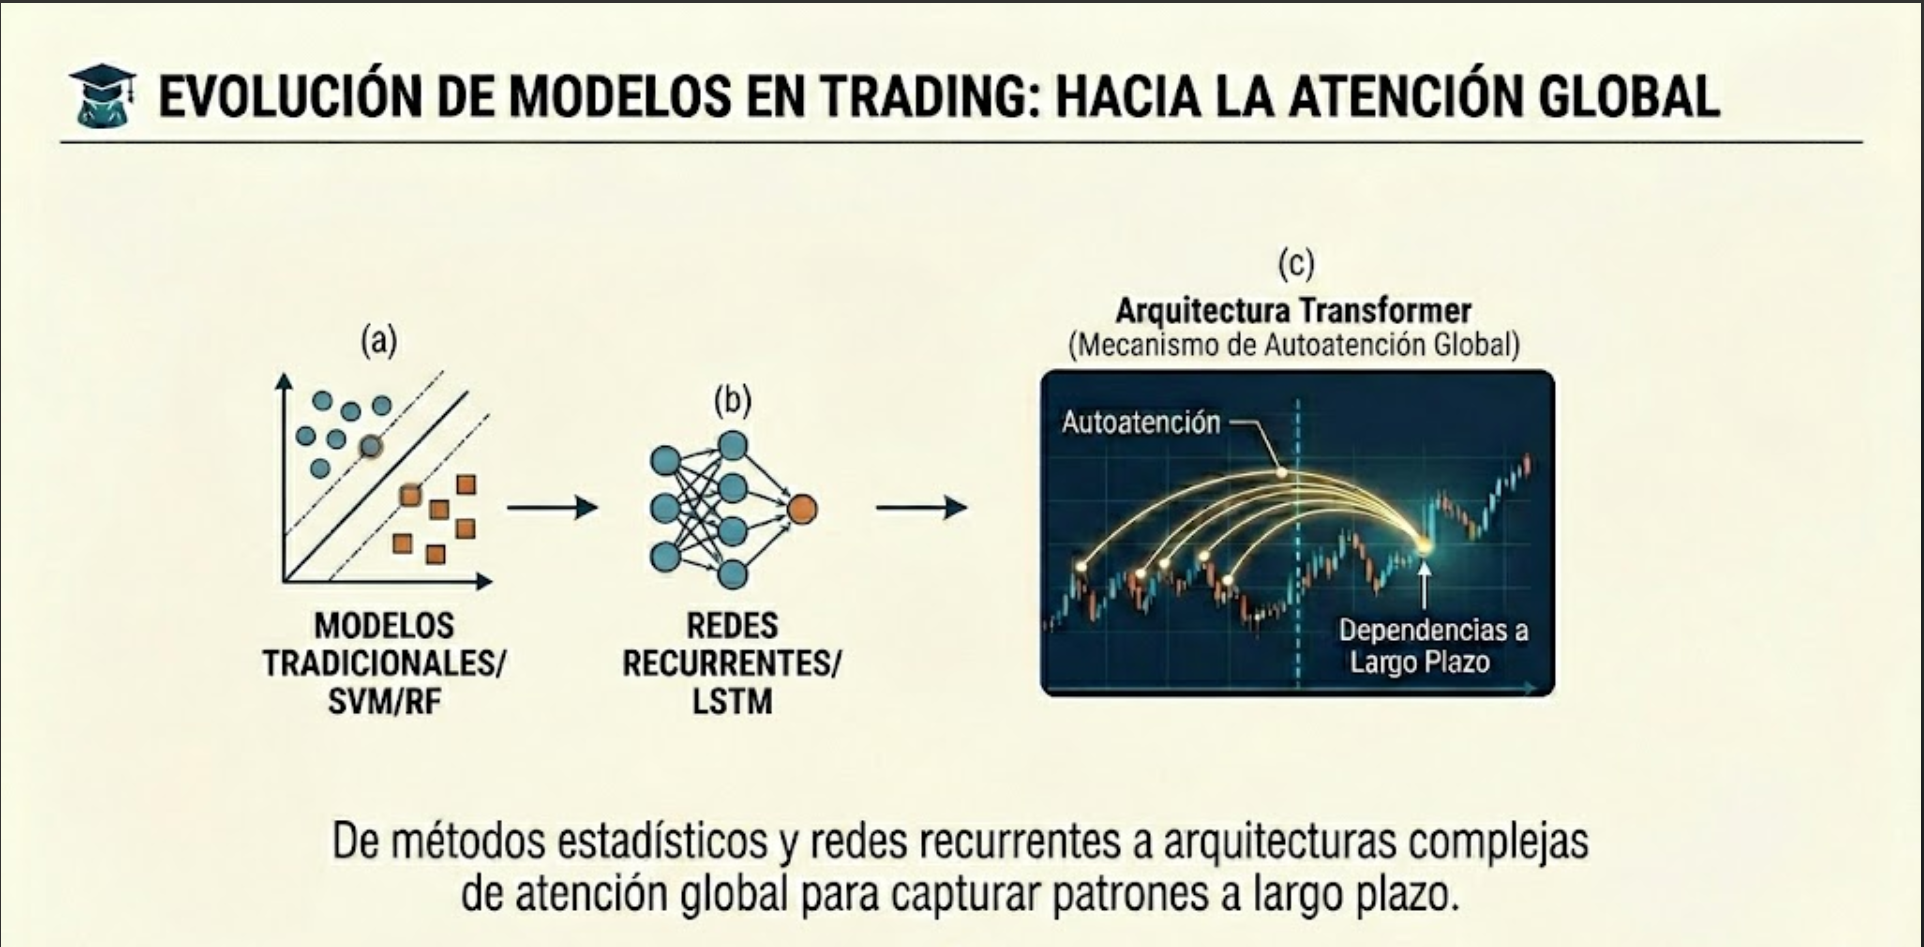
\includegraphics[width=0.95\textwidth, height=0.82\textheight, keepaspectratio]{evolucion-modelos.png}
\end{frame}

%--- 5 ---
\begin{frame}{Desafíos del dominio}
  \begin{columns}[T]
    \begin{column}{0.32\textwidth}
      \begin{tcolorbox}[familybox=coltrading, halign=center]
        {\large\faChartBar\; \textbf{Bajo SNR}}\\[0.4em]
        \normalsize Señal oculta\\bajo ruido aleatorio\\[0.3em]
        → riesgo de overfitting
      \end{tcolorbox}
    \end{column}
    \begin{column}{0.32\textwidth}
      \begin{tcolorbox}[familybox=colstat, halign=center]
        {\large\faChartLine\; \textbf{No estacionariedad}}\\[0.4em]
        \normalsize La distribución\\cambia con el tiempo\\[0.3em]
        → patrones no generalizan
      \end{tcolorbox}
    \end{column}
    \begin{column}{0.32\textwidth}
      \begin{tcolorbox}[familybox=colml, halign=center]
        {\large\faDollarSign\; \textbf{Costos de transacción}}\\[0.4em]
        \normalsize 0,1\% por trade\\consume ganancias\\[0.3em]
        → incluido en el backtest
      \end{tcolorbox}
    \end{column}
  \end{columns}
\end{frame}

%--- 6 ---
\begin{frame}{Objetivos}
  \large
  \begin{enumerate}
    \item[\faBook] Revisar el estado del arte: deep learning en finanzas
    \item[\faTerminal] Implementar un clasificador BTC/USDT con Transformer
    \item[\faFlask] Comparar \textbf{4 familias} de modelos con el mismo framework
    \item[\faUserCheck] Validar el modelo final con \textbf{CSCV} y \textbf{CPCV}
    \item[\faRobot] Desplegar un bot de trading operativo vía API Binance
  \end{enumerate}
\end{frame}

%========================================================================================
\section{Marco teórico}  % 7
%========================================================================================

%--- 8 ---
\begin{frame}{Trading y análisis técnico}
  \begin{columns}[T]
    \begin{column}{0.50\textwidth}
      \textbf{\faUsers\; Tipos de traders}\\[0.4em]
      \textit{Por duración:}
      \begin{itemize}
        \item \textbf{Scalping}: segundos o minutos
        \item \textbf{Diario}: intraday, sin overnight
        \item \textbf{Swing}: días a semanas
        \item \textbf{Eventos}: reacción a noticias
      \end{itemize}
      \vspace{0.3em}
      \textit{Por análisis:}\\[0.3em]
      \famtag{colstat}{Fundamental}\;
      \famtag{coltrans}{Técnico}\;
      \famtag{colml}{Algorítmico}\\[0.3em]
      \small Este trabajo: análisis \textbf{técnico algorítmico}
    \end{column}
    \begin{column}{0.47\textwidth}
      \textbf{\faListUl\; Indicadores usados}
      \large
      \begin{itemize}
        \item \textbf{Momentum}: RSI, ROC, Williams \%R
        \item \textbf{Tendencia}: MACD, ADX, Aroon
        \item \textbf{Volatilidad}: Bollinger Bands, Keltner
      \end{itemize}
    \end{column}
  \end{columns}
\end{frame}

%--- new — Indicadores técnicos ---
\begin{frame}{Indicadores técnicos}
  \begin{columns}[T]
    \begin{column}{0.54\textwidth}
      \small
      \begin{tabular}{ll}
        \toprule
        \textbf{Categoría} & \textbf{Indicadores} \\
        \midrule
        Momentum    & RSI, AO, Williams \%R, ROC \\
        Tendencia   & MACD, ADX, Aroon, CCI, Vortex \\
        Volatilidad & Bollinger, Keltner, Donchian \\
        Retornos    & \texttt{pct\_change}, retardos \\
        Embeddings  & Chronos → features tabulares \\
        \bottomrule
      \end{tabular}
      \vspace{0.5em}\\
      \small \textit{Selección}: MDI · MDA · SFI · ACF/PACF
    \end{column}
    \begin{column}{0.43\textwidth}
      \kpi{colml}{+25}{features por barra}
      \vspace{0.4em}
      \begin{tcolorbox}[familybox=fiubablue, top=3pt, bottom=3pt]
        \small \texttt{use\_pca=False}: correlaciones\\
        entre indicadores contienen señal
      \end{tcolorbox}
    \end{column}
  \end{columns}
\end{frame}

%--- 9 ---
\begin{frame}{Aprendizaje supervisado}
  \begin{columns}[T]
    \begin{column}{0.50\textwidth}
      \begin{itemize}
        \item[\faTasks] Tarea: \textbf{clasificación binaria} (no regresión)
        \item[\faChartBar] Métrica: \textbf{F1 ponderado} (clases desbalanceadas)
        \item[\faCogs] \textbf{Optuna}: búsqueda bayesiana eficiente
        \item[\faDatabase] Solo sobre datos de entrenamiento
        \item[\faCheckCircle] Holdout final: \textbf{una única evaluación}
      \end{itemize}
    \end{column}
    \begin{column}{0.47\textwidth}
      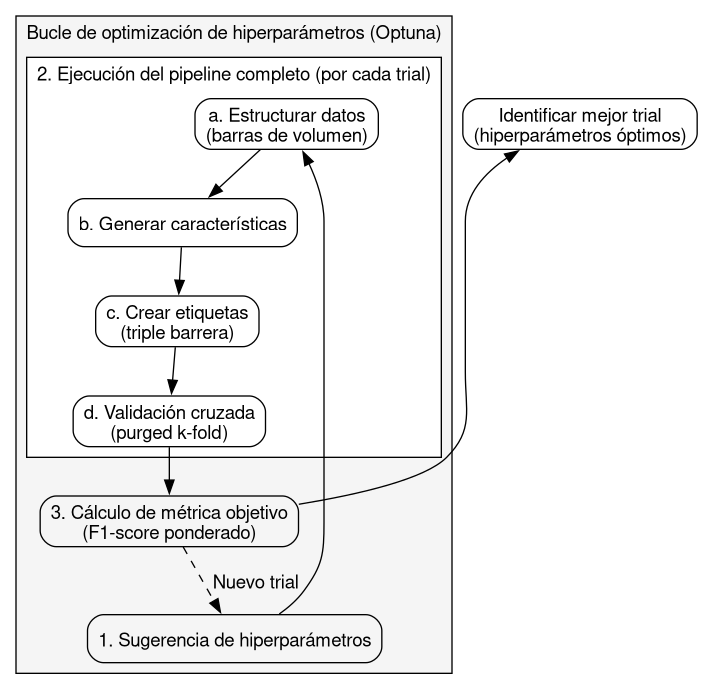
\includegraphics[width=\textwidth, height=0.62\textheight, keepaspectratio]{hyperparameter_pipeline.png}
    \end{column}
  \end{columns}
\end{frame}

%--- 10 ---
\begin{frame}{Chronos — Transformer para series de tiempo}
  \centering
  \includegraphics[width=0.92\textwidth, height=0.72\textheight, keepaspectratio]{chronos.png}\\[0.3em]
  \famtag{coltrans}{T5}\;
  \famtag{coltrans}{Bolt}\;
  \famtag{coltrans}{Chronos-2}
  \hfill{\tiny\textcolor{gray}{Ansari et al.\ (2024) — \textit{Chronos: Learning the Language of Time Series}}}
\end{frame}

%--- 11 ---
\begin{frame}{Etiquetado y validación sin data leakage}
  \begin{columns}[T]
    \begin{column}{0.50\textwidth}
      \textbf{\faTags\; Triple-barrier labeling}
      \begin{itemize}
        \item Barrera superior: objetivo de ganancia
        \item Barrera inferior: límite de pérdida
        \item Barrera temporal: expiración
        \item Adaptativa a la volatilidad dinámica
      \end{itemize}
      \vspace{0.4em}
      \textbf{\faFilter\; Purged K-Fold CV}
      \begin{itemize}
        \item K-Fold estándar: \alert{no válido} en series de tiempo
        \item Purgado + embargo (1–5\%)
      \end{itemize}
    \end{column}
    \begin{column}{0.47\textwidth}
      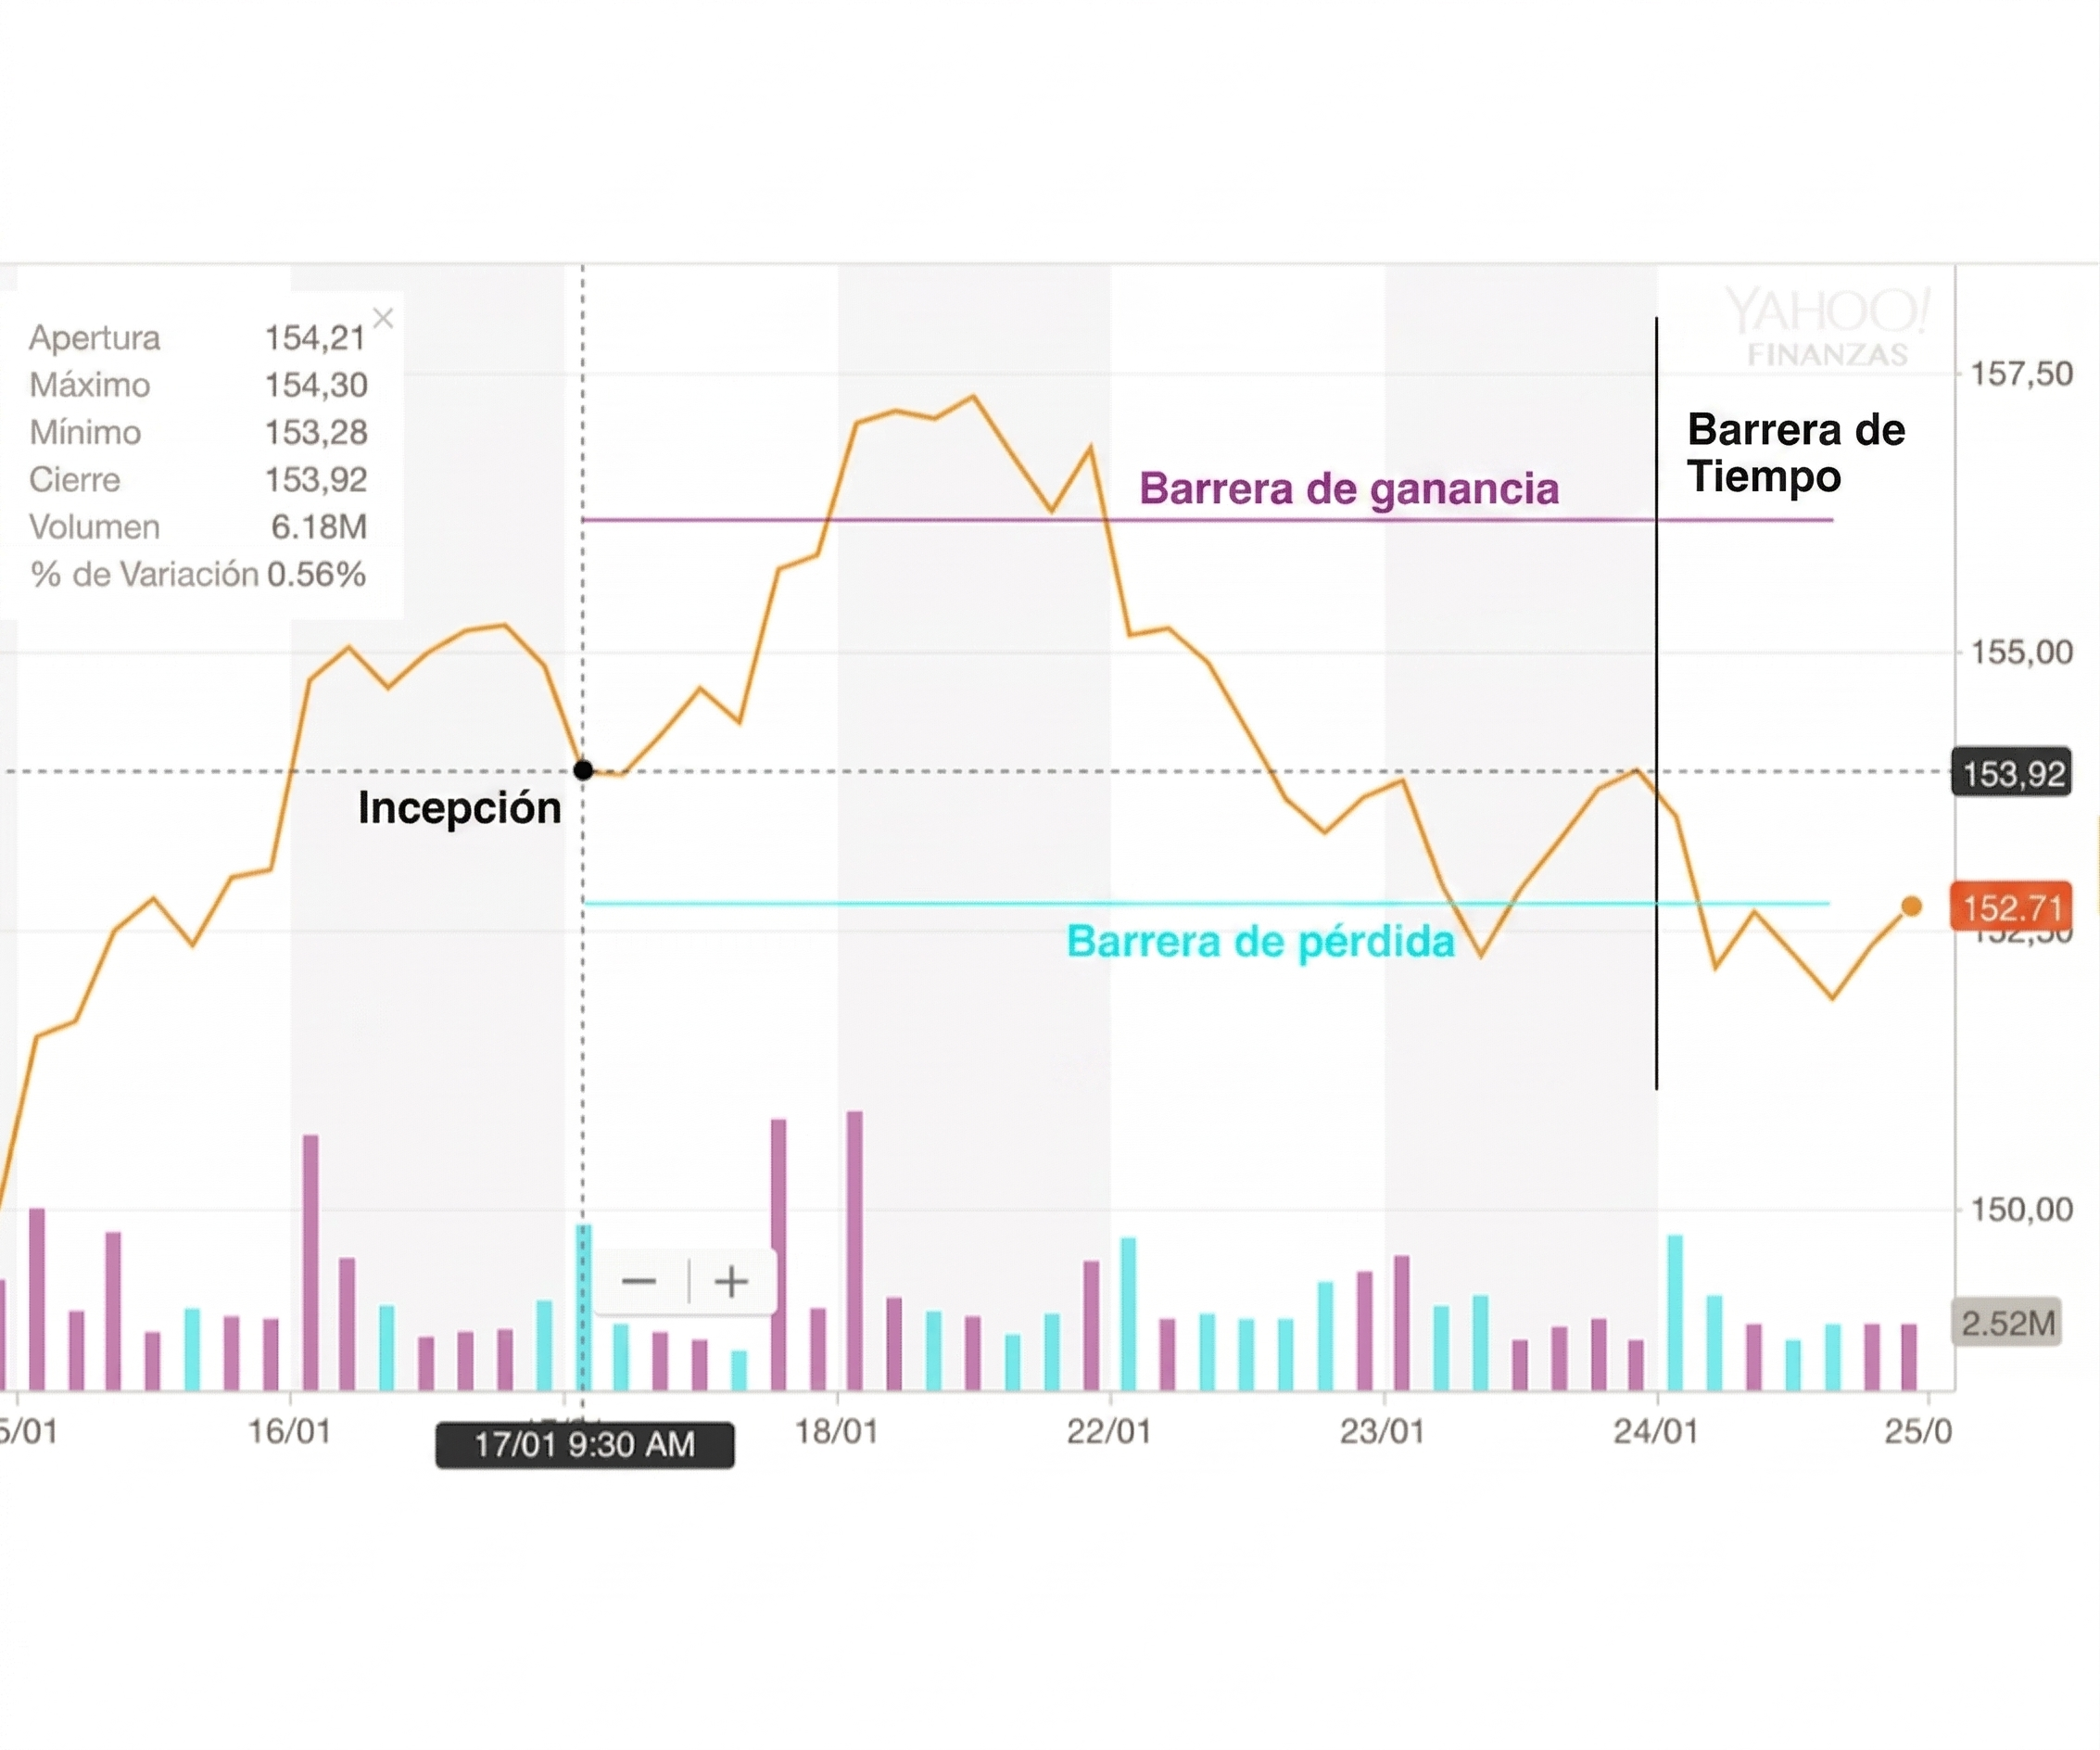
\includegraphics[width=\textwidth, height=0.58\textheight, keepaspectratio]{triple-barrier.png}
    \end{column}
  \end{columns}
\end{frame}

%--- 12 ---
\begin{frame}{Métricas de evaluación}
  \begin{columns}[T]
    \begin{column}{0.50\textwidth}
      \textbf{\faChartBar\; Rendimiento ajustado por riesgo}
      \begin{itemize}
        \item \textbf{Sharpe}: retorno / desviación estándar
        \item \textbf{Sortino}: solo volatilidad a la baja
        \item \textbf{Calmar}: retorno / max drawdown
        \item \textbf{PSR}: corrige asimetría y kurtosis
        \item \textbf{DSR}: penaliza búsqueda exhaustiva
      \end{itemize}
    \end{column}
    \begin{column}{0.47\textwidth}
      \begin{tcolorbox}[familybox=fiubablue]
        {\large\textbf{\faUserCheck\; Anti-overfitting}}\\[0.5em]
        \normalsize
        \textbf{PBO}: ¿ganó por azar?\\[0.3em]
        \textbf{CSCV}: estima PBO en $C$ combinaciones\\[0.3em]
        \textbf{CPCV}: $M$ caminos disjuntos\\
        → distribución del rendimiento OOS
      \end{tcolorbox}
    \end{column}
  \end{columns}
\end{frame}

%========================================================================================
\section{Datos y preprocesamiento}  % 13
%========================================================================================

%--- 14 ---
\begin{frame}{Pipeline de datos}
  \begin{columns}[T]
    \begin{column}{0.50\textwidth}
      \begin{enumerate}
        \item \textbf{Klines 1 min} — Binance, 2020–2025
        \item \textbf{Barras de volumen} (50 000 uBTC) — ↓ autocorrelación
        \item \textbf{Diferenciación fraccional} ($d{\approx}0{,}4$) — ADF 95\%
        \item \textbf{Indicadores técnicos}: RSI, Bollinger, MACD…
        \item \textbf{StandardScaler} — ajustado solo en train
        \item \textbf{Triple-barrier labeling} ($\tau{>}0{,}98$)
      \end{enumerate}
    \end{column}
    \begin{column}{0.47\textwidth}
      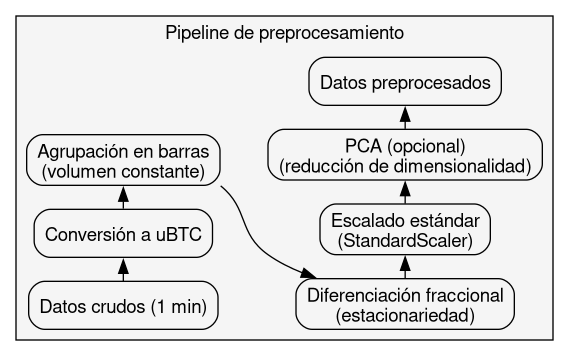
\includegraphics[width=\textwidth, height=0.62\textheight, keepaspectratio]{preprocessing_pipeline.png}
    \end{column}
  \end{columns}
\end{frame}

%--- new — Barras de volumen ---
\begin{frame}{Barras de volumen — Muestreo adaptativo}
  \begin{columns}[T]
    \begin{column}{0.50\textwidth}
      \textbf{Barras de tiempo (1 min)}
      \begin{itemize}
        \item[$\boldsymbol{\times}$] Muestreo uniforme en el tiempo
        \item[$\boldsymbol{\times}$] Satura en baja actividad de mercado
      \end{itemize}
      \vspace{0.5em}
      \textbf{\textcolor{coltrans}{\faCheckCircle}\; Barras de volumen (50k uBTC)}
      \begin{itemize}
        \item Proporcional a la actividad real
        \item Menor autocorrelación y heterocedasticidad
        \item Mayor resolución en períodos volátiles
      \end{itemize}
    \end{column}
    \begin{column}{0.47\textwidth}
      \centering
      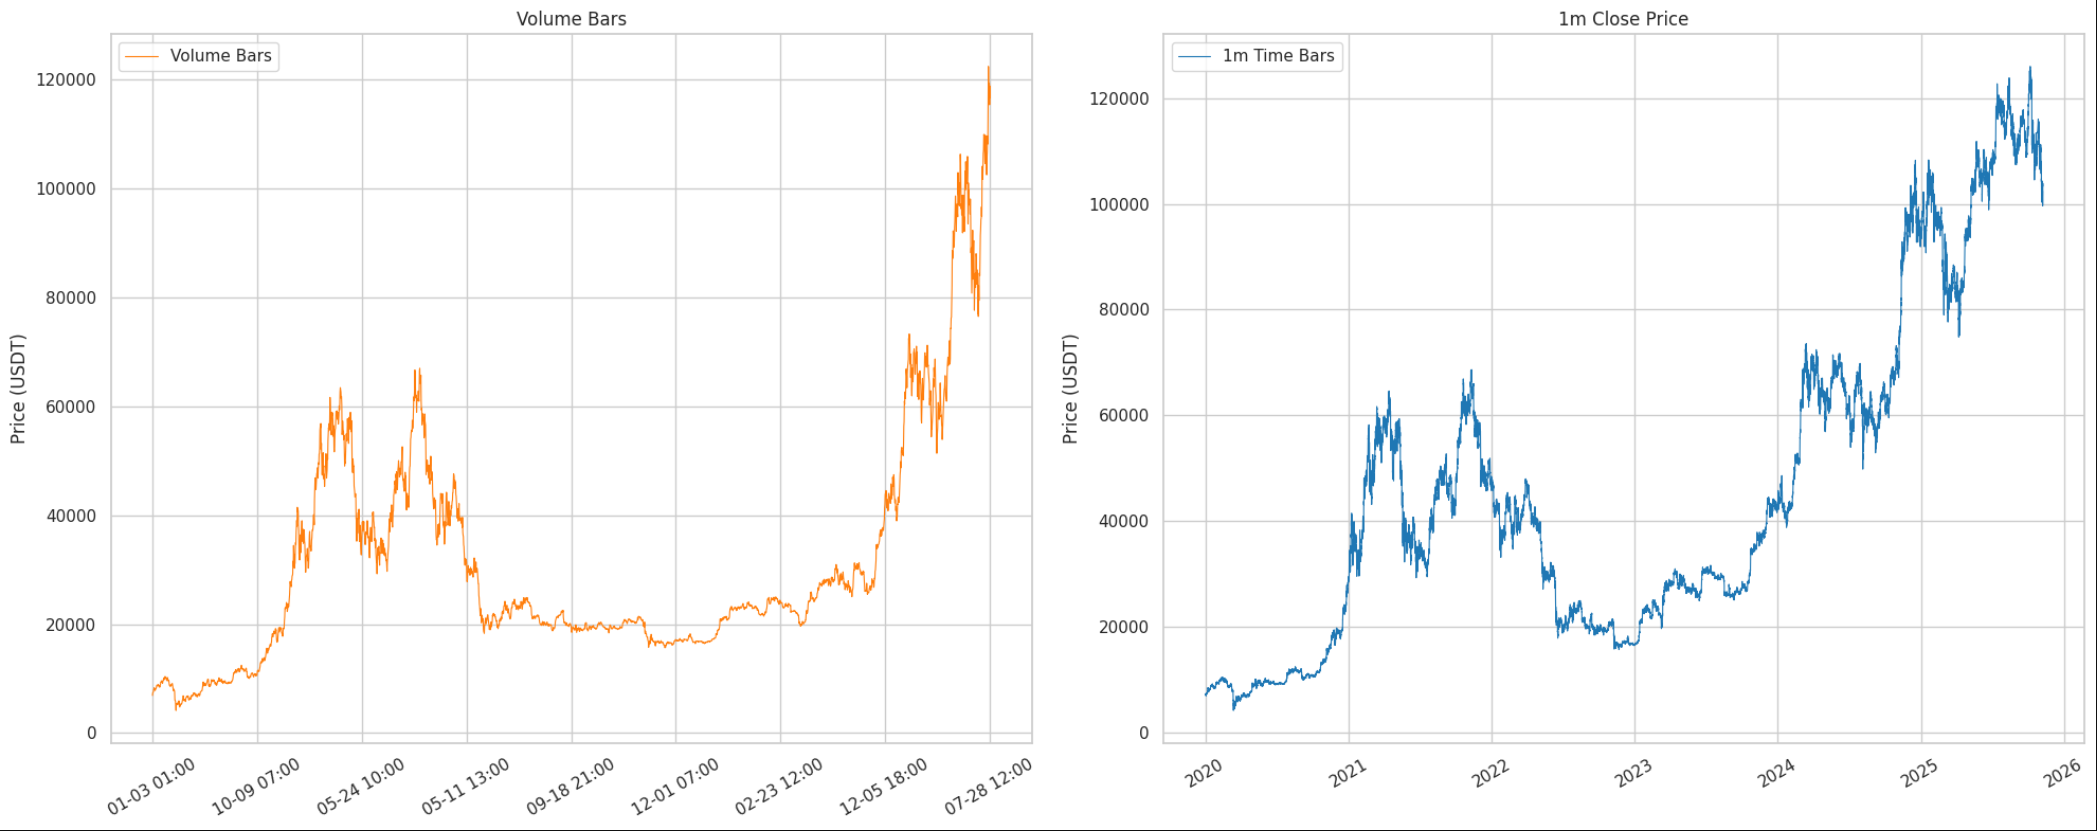
\includegraphics[width=\textwidth, height=0.72\textheight, keepaspectratio]{bars-vs-1m.png}
    \end{column}
  \end{columns}
\end{frame}

\begin{frame}{Bot de trading — Arquitectura}
  \begin{columns}[T]
    \begin{column}{0.44\textwidth}
      \begin{itemize}
        \item[\faCogs] \textbf{Orquestador}: instancia módulos
        \item[\faRobot] \textbf{Motor}: recolectar→predecir→actuar
        \item[\faDatabase] \textbf{Exchange}: API Binance real o mock
        \item[\faChartLine] \textbf{Estrategia}: Modelo configurado → señal
      \end{itemize}
      \vspace{0.4em}
      \begin{tcolorbox}[familybox=coltrans, top=2pt, bottom=2pt]
        \footnotesize Stop-loss · monitoreo Flask\\
        Desplegado en Binance (producción)
      \end{tcolorbox}
    \end{column}
    \begin{column}{0.53\textwidth}
      \centering
      \begin{tikzpicture}[scale=0.92,
        box/.style={draw, rounded corners=3pt, font=\small,
                    inner sep=4pt, minimum width=2.1cm, minimum height=0.50cm},
        arr/.style={-{Stealth}, thin}
      ]
        %── Orquestador ───────────────────────────
        \node[box, draw=fiubablue, fill=fiubablue!10,
              minimum width=4.4cm] (orch) at (2.2, 4.0)
          {\faCogs\ Orquestador};

        %── Motor ─────────────────────────────────
        \node[box, draw=fiubablue!60, fill=fiubablue!6,
              minimum width=4.4cm] (motor) at (2.2, 3.0)
          {\faRobot\ Motor del bot};
        \draw[arr, fiubablue!55] (orch) -- (motor);

        %── Exchange (left) ───────────────────────
        \node[box, draw=colml, fill=colml!10] (exch) at (0.8, 1.75)
          {\faDatabase\ Exchange};
        % Arrow from left side of Motor bottom
        \draw[arr, fiubablue!50]
          ($(motor.south)+(-0.85,0)$) -- (exch.north);

        %── Estrategia (right) ────────────────────
        \node[box, draw=coltrans, fill=coltrans!10] (strat) at (3.8, 1.75)
          {\faChartLine\ Estrategia};
        % Arrow from right side of Motor bottom
        \draw[arr, fiubablue!50]
          ($(motor.south)+(+0.85,0)$) -- (strat.north);

        %── BTC/USDT ──────────────────────────────
        \node[box, draw=accent, fill=accent!8] (mkt) at (0.8, 0.60)
          {BTC/USDT};
        \draw[arr, colml!65] (exch) -- (mkt);
        \draw[arr, accent!50, bend right=40] (mkt) to (exch);

        %── Señal: Estrategia → Motor (right side) ─
        \draw[arr, coltrans!65]
          (strat.north) 
        -- ($(motor.south)+(+0.85,0)$);
        \node[font=\small\bfseries, coltrans!75!black, anchor=west]
          at ($(strat.east)+(0.38,0.76)$) {señal};
      \end{tikzpicture}
    \end{column}
  \end{columns}
\end{frame}

%========================================================================================
\section{Experimentos y resultados}  % 15
%========================================================================================

%--- 16 ---
\begin{frame}{Algoritmos de trading clásicos}
  \begin{columns}[T]
    \begin{column}{0.50\textwidth}
      \begin{tcolorbox}[familybox=coltrading]
        \begin{tabular}{lcc}
          \toprule
          \textbf{Clasificador} & \textbf{F1} & \textbf{Std} \\
          \midrule
          BollingerBands  & 0,511 & 0,022 \\
          RSIDivergence   & 0,508 & 0,001 \\
          MaCrossover     & 0,501 & 0,002 \\
          MACD            & 0,499 & 0,002 \\
          SmaCross        & 0,498 & 0,002 \\
          \bottomrule
        \end{tabular}
      \end{tcolorbox}
    \end{column}
    \begin{column}{0.47\textwidth}
      \begin{itemize}
        \item[\faTimes] Ninguno supera F1 $= 0{,}51$
        \item[\faCheckCircle] RSIDivergence: std $= 0{,}001$ — más confiable
        \item[\faExclamationTriangle] BollingerBands: mayor techo, mayor riesgo
        \item[\faSearch] 6 clasificadores · 184 trials
      \end{itemize}
      \vspace{0.3em}
      \begin{tcolorbox}[familybox=accent, top=2pt, bottom=2pt]
        \normalsize\textbf{El análisis técnico simple no captura señal}
      \end{tcolorbox}
    \end{column}
  \end{columns}
\end{frame}

%--- 18 ---
\begin{frame}{Modelos estadísticos — ARIMA, GARCH, Kalman}
  \begin{columns}[T]
    \begin{column}{0.50\textwidth}
      \begin{tcolorbox}[familybox=colstat]
        \begin{tabular}{lcc}
          \toprule
          \textbf{Modelo} & \textbf{F1 máx} & \textbf{Std} \\
          \midrule
          ARIMA           & 0,500 & 0,118 \\
          ARIMA-GARCH     & 0,495 & 0,116 \\
          SARIMA          & 0,486 & 0,046 \\
          Kalman-ARIMA    & 0,418 & 0,165 \\
          \bottomrule
        \end{tabular}
      \end{tcolorbox}
    \end{column}
    \begin{column}{0.47\textwidth}
      \begin{itemize}
        \item[\faTimes] Ninguno supera el azar
        \item[\faArrowDown] Más complejidad = peor resultado
        \item[\faExclamationTriangle] Std 0,118 → fallas catastróficas (F1 → 0)
        \item[\faKey] \texttt{threshold} $\approx 10^{-6}$, corr $= -0{,}93$
      \end{itemize}
      \vspace{0.3em}
      \begin{tcolorbox}[familybox=accent, top=2pt, bottom=2pt]
        \normalsize PBO $= 0$: \textbf{consistentemente al nivel del azar}
      \end{tcolorbox}
    \end{column}
  \end{columns}
\end{frame}

%--- 19 ---
\begin{frame}{Machine Learning — XGBoost y AutoGluon}
  \begin{columns}[T]
    \begin{column}{0.50\textwidth}
      \begin{tcolorbox}[familybox=colml]
        \begin{tabular}{lcc}
          \toprule
          \textbf{Algoritmo} & \textbf{F1 máx} & \textbf{n} \\
          \midrule
          XGBoost Palazzo   & 0,647 & 60 \\
          AutoGluon Palazzo & 0,639 & 20 \\
          \bottomrule
        \end{tabular}
        \vspace{0.2em}\\
        \small\texttt{max\_depth=4 · lr=0,003 · n\_est=373}\\
        Mejor AutoGluon: \texttt{LightGBMXT\_BAG\_L1}
      \end{tcolorbox}
    \end{column}
    \begin{column}{0.47\textwidth}
      \begin{itemize}
        \item[\faArrowUp] F1: $0{,}50 \to 0{,}65$ — primer salto real
        \item[\faHourglass] AutoGluon: misma calidad, 10× más lento
        \item[\faMinusCircle] PCA no aporta en ningún trial
        \item[\faCheckCircle] $\tau{>}0{,}98$: etiquetas menos frecuentes, más limpias
      \end{itemize}
      \vspace{0.3em}
      \begin{tcolorbox}[familybox=colml]
        \small PBO $= 0{,}486$ — selección moderada
      \end{tcolorbox}
    \end{column}
  \end{columns}
\end{frame}

%--- 20 ---
\begin{frame}{Transformer — 3 familias Chronos}
  \begin{tabular}{llcc}
    \toprule
    \textbf{Familia} & \textbf{Pipeline} & \textbf{F1 máx} & \textbf{Std} \\
    \midrule
    \famtag{coltrans}{Embeddings} & ChronosFeature T5-small  & 0,633 & 0,022 \\
    \famtag{coltrans}{Embeddings} & ChronosBoltFeature        & 0,628 & 0,008 \\
    \famtag{colstat}{Meta-etiquetado} & ChronosMetaLabeling  & 0,657 & ---  \\
    \rowcolor{coltrans!15}
    \famtag{coltrans}{Fine-tuning} & \textbf{FinetuneToClass (Chronos-2)} & \textbf{0,819} & --- \\
    \bottomrule
  \end{tabular}
  \vspace{0.5em}
  \begin{columns}[T]
    \begin{column}{0.48\textwidth}
      \begin{tcolorbox}[familybox=colstat, top=2pt, bottom=2pt]
        \small Meta-filtro: degrada el F1 en 6 de 8 runs
      \end{tcolorbox}
    \end{column}
    \begin{column}{0.48\textwidth}
      \begin{tcolorbox}[familybox=coltrans, top=2pt, bottom=2pt]
        \small Fine-tuning end-to-end: \textbf{+0,16 F1} sobre embeddings
      \end{tcolorbox}
    \end{column}
  \end{columns}
\end{frame}

\begin{frame}{Resumen — 4 familias de modelos}
  \begin{columns}[T]
    \begin{column}{0.55\textwidth}
      \begin{tikzpicture}
        \begin{axis}[
          xbar,
          width=\textwidth,
          height=5cm,
          bar width=0.45cm,
          xlabel={\small F1 OOS},
          xlabel style={font=\small},
          ytick={1,2,3,4},
          yticklabels={
            \famtag{coltrading}{Trading},
            \famtag{colstat}{Estadístico},
            \famtag{colml}{ML},
            \famtag{coltrans}{Transformer}
          },
          yticklabel style={font=\small},
          xmin=0.40, xmax=0.93,
          xtick={0.50,0.60,0.70,0.80},
          xticklabel style={font=\small},
          nodes near coords,
          nodes near coords style={font=\footnotesize\bfseries},
          nodes near coords align={horizontal},
          enlarge y limits=0.25,
          axis line style={draw=none},
          tick style={draw=none},
        ]
          \addplot[fill=coltrading!80, draw=coltrading!50!black, bar shift=0pt] coordinates {(0.50,1)};
          \addplot[fill=colstat!80,    draw=colstat!50!black,    bar shift=0pt] coordinates {(0.504,2)};
          \addplot[fill=colml!80,      draw=colml!50!black,      bar shift=0pt] coordinates {(0.656,3)};
          \addplot[fill=coltrans!80,   draw=coltrans!50!black,   bar shift=0pt] coordinates {(0.819,4)};
        \end{axis}
      \end{tikzpicture}
    \end{column}
    \begin{column}{0.42\textwidth}
      \vspace{1.5em}
      \kpi{coltrans}{0,819}{F1 OOS — Transformer}
      \vspace{0.5em}
      \kpi{accent}{$+0{,}16$}{Brecha vs.\ 2° mejor}
      \vspace{0.8em}
      \normalsize Mismo framework · mismos datos · misma métrica
    \end{column}
  \end{columns}
\end{frame}

%--- 21 ---
\begin{frame}{Selección del modelo — CSCV cruzado}
  \begin{columns}[T]
    \begin{column}{0.52\textwidth}
      \begin{tabular}{lcc}
        \toprule
        \textbf{Experimento} & \textbf{IS} & \textbf{OOS} \\
        \midrule
        \rowcolor{coltrans!15}
        \textbf{FinetuneToClass} & \textbf{98,6\%} & \textbf{98,6\%} \\
        Finetuned\_Feature   & 1,4\%  & 1,4\%  \\
        Resto (5 exp.)       & 0\%    & 0\%    \\
        \bottomrule
      \end{tabular}
      \vspace{0.5em}\\
      \small $N{=}203$ trials, $C{=}70$ combinaciones, PBO $= 0$
    \end{column}
    \begin{column}{0.45\textwidth}
      \kpi{coltrans}{0,819}{F1 OOS — modelo final}
      \vspace{0.5em}
      \begin{tcolorbox}[familybox=coltrans]
        \small\texttt{chronos-2-small}\\
        $\tau = 0{,}910$\\
        \texttt{volume\_threshold} $= 45\,988$
      \end{tcolorbox}
    \end{column}
  \end{columns}
\end{frame}

%--- 22 ---
\begin{frame}{Validación final — CPCV (5 caminos disjuntos)}
  \begin{columns}[T]
    \begin{column}{0.42\textwidth}
      \large
      \begin{tabular}{cc}
        \toprule
        \textbf{Camino} & \textbf{F1} \\
        \midrule
        1 & 0,8219 \\
        2 & 0,8235 \\
        3 & 0,8221 \\
        \rowcolor{coltrans!15} 4 & \textbf{0,8303} \\
        \rowcolor{coltrans!15} 5 & \textbf{0,8277} \\
        \midrule
        \textbf{Media} & $0{,}825 \pm 0{,}003$ \\
        \bottomrule
      \end{tabular}
    \end{column}
    \begin{column}{0.55\textwidth}
      \begin{itemize}
        \item[\faCheckCircle] Std $= 0{,}003$ — rendimiento estable
        \item[\faCheckCircle] Caminos 4 y 5 (más recientes) no caen
        \item[\faCheckCircle] F1 CPCV $(0{,}825)$ $>$ F1 Optuna $(0{,}818)$
        \item[\faCheckCircle] 17 330 predicciones OOS totales
      \end{itemize}
      \vspace{0.3em}
      \kpi{coltrans}{$0{,}825 \pm 0{,}003$}{F1 medio CPCV — sin sobreajuste}
    \end{column}
  \end{columns}
\end{frame}

%========================================================================================
\section{Conclusiones}  % 23
%========================================================================================

%--- 24 ---
\begin{frame}{Conclusiones y próximos pasos}
  \begin{columns}[T]
    \begin{column}{0.50\textwidth}
      \textbf{\faCheckCircle\; Logros}
      \begin{itemize}
        \item Pipeline completo: 3M+ filas BTC/USDT
        \item ARIMA y trading clásico: nivel del azar
        \item XGBoost: primer salto real (F1 $= 0{,}65$)
        \item \alert{Chronos fine-tuning: F1 $= 0{,}819$, validado}
        \item Bot operativo con stop-loss automático
      \end{itemize}
    \end{column}
    \begin{column}{0.47\textwidth}
      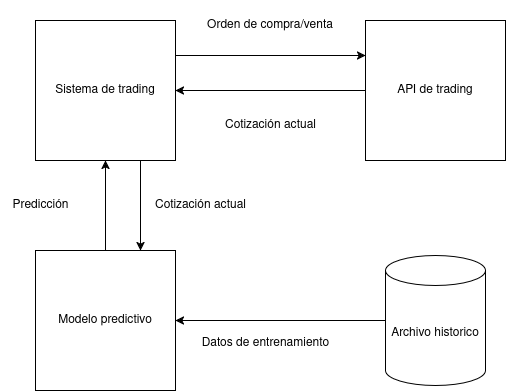
\includegraphics[width=\textwidth, height=0.45\textheight, keepaspectratio]{bloques-tp-final.drawio.png}
      \vspace{0.2em}\\
      \textbf{\faArrowRight\; Próximos pasos}\\[0.1em]
      \small Bet sizing · Ensamble · HRP · Microestructura
    \end{column}
  \end{columns}
\end{frame}

%--- 25 — Demo ---
\begin{frame}{Demostración — Bot en producción}
  \centering
  \vspace{0.3em}
  {\large\faRobot\;\textbf{Bot operativo en Binance}}\\[0.9em]
  \begin{tcolorbox}[familybox=coltrans, top=8pt, bottom=8pt,
                    left=16pt, right=16pt, halign=center]
    {\large\ttfamily [URL DEL VIDEO]}
  \end{tcolorbox}
  \vspace{0.7em}
  \begin{columns}[T]
    \begin{column}{0.30\textwidth}
      \centering{\Large\textcolor{fiubablue}{\faDatabase}}\\[0.3em]
      \small Datos Binance\\en tiempo real
    \end{column}
    \begin{column}{0.30\textwidth}
      \centering{\Large\textcolor{coltrans}{\faChartLine}}\\[0.3em]
      \small Señal Chronos\\BTC \(\leftrightarrow\) USDT
    \end{column}
    \begin{column}{0.30\textwidth}
      \centering{\Large\textcolor{accent}{\faBell}}\\[0.3em]
      \small Monitoreo Flask\\+ stop-loss
    \end{column}
  \end{columns}
\end{frame}

%--- 25 ---
{\setbeamercolor{background canvas}{bg=fiubablue}
\begin{frame}[plain]
  \centering\vspace{2em}
  \color{white}
  \Large\textbf{¡Gracias!}\\[1.5em]
  \normalsize
  Ing. Martín Leonardo Centurión\\[0.5em]
  \texttt{centurionm.leo@gmail.com}\\[2em]
  \large\textit{¿Preguntas?}
\end{frame}}

%========================================================================================
\appendix
%========================================================================================

\begin{frame}[noframenumbering]{Respaldo — Hiperparámetros XGBoost Palazzo}
  \begin{tabular}{ll}
    \toprule
    \textbf{Parámetro} & \textbf{Valor} \\
    \midrule
    \texttt{max\_depth}        & 4       \\
    \texttt{learning\_rate}    & 0,00328 \\
    \texttt{n\_estimators}     & 373     \\
    \texttt{tau}               & 1,261   \\
    \texttt{volume\_threshold} & 28 522  \\
    \texttt{use\_pca}          & False   \\
    \bottomrule
  \end{tabular}
\end{frame}

\begin{frame}[noframenumbering]{Respaldo — Hiperparámetros modelo final Chronos}
  \begin{tabular}{ll}
    \toprule
    \textbf{Parámetro} & \textbf{Valor} \\
    \midrule
    Modelo base                 & \texttt{autogluon/chronos-2-small} \\
    $\tau$                      & 0,910   \\
    \texttt{volume\_threshold}  & 45 988  \\
    \texttt{prediction\_length} & 2       \\
    \texttt{pct\_embargo}       & 0,05    \\
    \texttt{n\_splits}          & 3       \\
    \bottomrule
  \end{tabular}
\end{frame}

\begin{frame}[noframenumbering]{Respaldo — Sensibilidad modelos estadísticos}
  \begin{tabular}{llcp{5cm}}
    \toprule
    \textbf{Modelo} & \textbf{Parámetro} & \textbf{Corr} & \textbf{Interpretación} \\
    \midrule
    ARIMA-family    & threshold   & $-0{,}93$ & Umbral cercano a cero es crítico \\
    ARIMAXGARCH     & threshold   & $-0{,}99$ & Umbrales altos degradan el modelo \\
    ARIMAClassifier & lookback    & $-0{,}37$ & Historial corto (720 h) preferido \\
    ARIMAXGARCH     & $q$ (MA)    & $+0{,}85$ & Orden MA alto es mejor \\
    \bottomrule
  \end{tabular}
\end{frame}

\begin{frame}[noframenumbering]{Respaldo — Barras de volumen vs. barras temporales}
  \begin{columns}[T]
    \begin{column}{0.50\textwidth}
      \textbf{Barras de tiempo (1 min)}
      \begin{itemize}
        \item Muestreo uniforme en el tiempo
        \item Alta autocorrelación en baja actividad
      \end{itemize}
      \vspace{0.5em}
      \textbf{Barras de volumen (50 000 uBTC)}
      \begin{itemize}
        \item Muestreo por actividad real
        \item Menor autocorrelación y heterocedasticidad
        \item Mayor resolución en alta volatilidad
      \end{itemize}
    \end{column}
    \begin{column}{0.47\textwidth}
      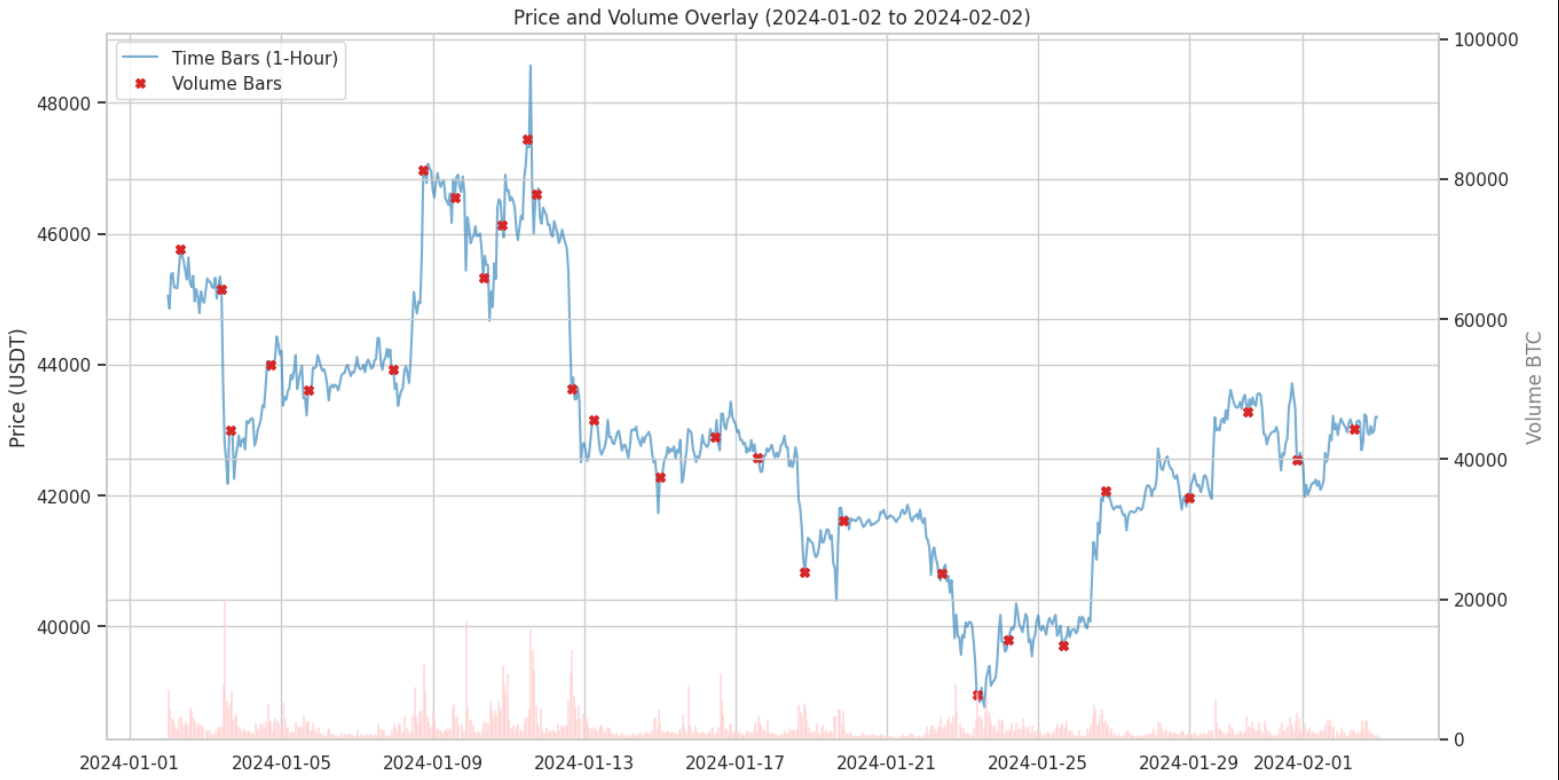
\includegraphics[width=\textwidth]{bars-volume-1m.png}
    \end{column}
  \end{columns}
\end{frame}

\begin{frame}[noframenumbering]{Respaldo — Diferenciación fraccional}
  \begin{columns}[T]
    \begin{column}{0.55\textwidth}
      \begin{itemize}
        \item $d=1$: serie de retornos — elimina demasiada memoria
        \item $d=0$: precio original — no estacionario
        \item $d \approx 0{,}4$: mínimo que garantiza estacionariedad (ADF 95\%)
      \end{itemize}
      \vspace{0.5em}
      \begin{tcolorbox}[familybox=fiubablue]
        Preserva la mayor cantidad de contexto\\
        histórico posible sin violar estacionariedad
      \end{tcolorbox}
    \end{column}
    \begin{column}{0.42\textwidth}
      \begin{tcolorbox}[familybox=coltrading]
        \centering
        {\Large\bfseries $d = 0{,}4$}\\[0.3em]
        Punto óptimo entre\\
        memoria e información
      \end{tcolorbox}
    \end{column}
  \end{columns}
\end{frame}

%----------------------------------------------------------------------------------------
\end{document}
